\section{Mechanics}
% In this section briefly describe the software and hardware of the robot
\setlength\intextsep{0pt}
In the past two years there were multiple changes applied to the chip kicker in order to reach the most efficient design. A great number of simulation tests were done on every chip design and after a successful test, the parts were manufactured for real world testing procedures.

\subsection{Chip kickers new design}
Chip kicker is a part which should have a high resistance against impacts, it has to be efficient in transmitting the force applied to it from the chip kickers plunger to the ball. The first improvement in the chip kicker is that $\theta$ (angle between a line which passes through the chip kickers axis of rotation and impact point and the direction of the force vector)has been increased to 90 degrees. With this improvement the force applied to the chip kicker will be completely in the direction of the angular acceleration of the chip kicker. According to the torque relation, It is shown that when the angle between the force and the distance vector turn into 90 degrees, the ball would receive the most impact from that force.\\
\indent The other improvement is to increase the moment of inertia around the chip kickers axis of rotation. This way, more angular acceleration can be achieved by the chip kicker.\\
\indent In this section a function for angular acceleration of the chip kicker will be driven. As known, the relation between the moment of inertia around the chip kickers axis of rotation and sum of torque applied to the chip kicker can be written as:
\begin{equation} 
\label{eq:1}
\sum T=I\alpha
\end{equation}
\begin{equation}
\label{eq:2}
T=Fb
\end{equation}
Equation \ref{eq:1} is one of the general equations of motion for rigid body in plane motion [7]. Although the chip kicker is a 3D model in real life but the most important part of the chip kicker (which is shown in Fig.\ref{fig:CHIP_SIDE_VIEW}) is the design of the arms of the chip kicker which can be discussed in 2D (The arms of the chip kicker which is shown in Fig.\ref{fig:CHIP_SIDE_VIEW} are the same at both left and right sides of the chip kicker assembly. For 2D analysis we neglect the thickness of this part).\\
\\
$b$ is the vertical distance between center of pin of the chip kicker and point which force is applied.\\
\\
$T$ is torques applied to the chip kicker. In this problem there is only one torque which is applied to the chip kicker and in equation \ref{eq:2} this torque is defined.\\
\\
$\alpha$ is the angular acceleration of the chip kicker.\\
\\
$I$ is moment of inertia around the axis of rotation of the chip kicker.\\
\\
$F$ is the force applied to the chip kicker by the plunger.\\
\\
It is not necessary to calculate the impact force accurately thus, it is assumed that the force applied, is constant to reduce the parameters involved in the new chip kickers design. the impact force is approximated by the equation below:
\begin{equation}
F=\dfrac{m\limits_{plunger} {V}^2\limits_{f-plunger}}{2d}
\end{equation}
Where $m\limits_{plunger}$ is the mass of the plunger and ${V}\limits_{f-plunger}$ is the velocity of plunger exactly before the impact and $d$ is the distance in which the plunger and the chip kicker are in contact during the impact.\\
\indent Below is an expression for the angular acceleration, resulted from the previous equations:
\begin{equation}
\alpha = \dfrac{b m\limits_{plunger} {V}^2\limits_{f-plunger}}{2Id}
\end{equation}
By assuming F as constant\footnote{Constant force assumption is because of the very low period of time which the plunger and chip kicker is in contact. It is assume that the force won’t change significantly during the impact.}
, The angular acceleration will be a function of:
\begin{equation}
\alpha=f(\dfrac{b}{I})
\end{equation}
As a result, if the moment of inertia around the axis of rotation reduces by decreasing the mass of the chip kicker or reducing the distance between its center of mass and the axis of rotation, $\alpha$ will increase.
As shown in Fig.\ref{fig:CHIP_SIDE_VIEW}, $\dfrac{b}{I}$ is calculated for both old and new designs:\\
\begin{figure}
	\centering
	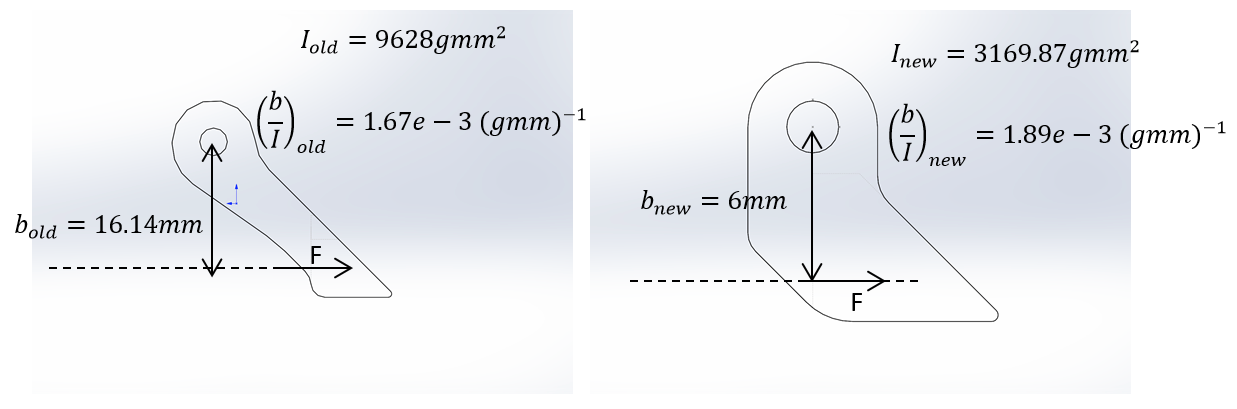
\includegraphics[width=1.0\textwidth]{images/SIDE_VIEW_CHIP.png}
	\caption{$\dfrac{b}{I}$ for old (left) and new (right) design}
	\label{fig:CHIP_SIDE_VIEW}
\end{figure}\\
The results show that $\dfrac{b}{I}$ for the new design is larger than the old one; Therefore, the angular acceleration for the new design should be more than the angular acceleration in the old design. As discussed above, the new design of the chip kicker is more simpler to manufacture ,more reliable and lighter than the old design. %Including these improvements, it also has higher angular acceleration which means reducing its weight won’t affect its functionality.\\
\\
\indent In order to test these results, the impact for both old and new designs were simulated in SolidWorks (as shown in Fig.\ref{fig:SIM2CHIP}).\\
\begin{figure}
	\centering
	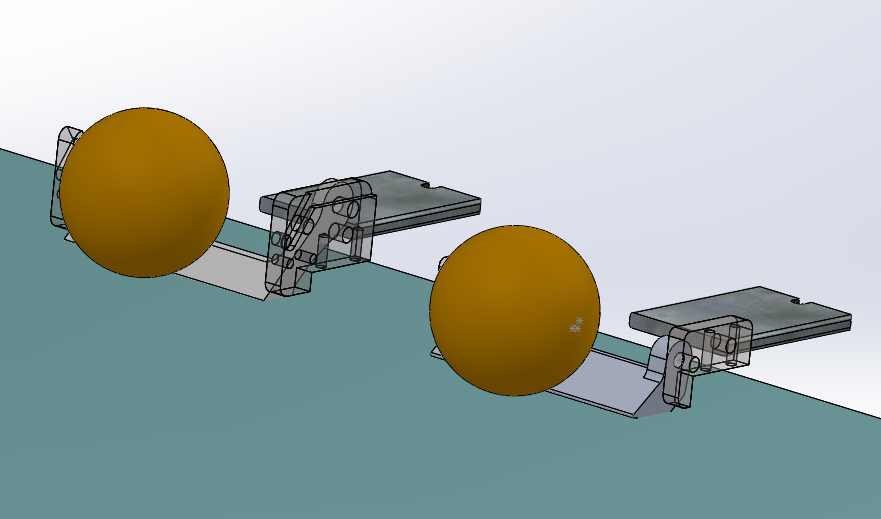
\includegraphics[width=0.8\textwidth]{images/SIM_CHIPx2.png}
	\caption{A view of the old (top left)and new (bottom right)chip kickers in a simulation enviroment}
	\label{fig:SIM2CHIP}
\end{figure}\\
\\
For simulating ball kick in \textit{SolidWorks Motion analysis} The below steps were taken:
\begin{enumerate}
  \item Creation of the part of the SSL field.
  \item Importing the necessary parts of the new and old designs of the chip kicker into the assembly.
  \item Fixing the left and right stands of the chip kickers for both designs by using the “Fix” option in SolidWorks (in reality the left and right stands of the chip kickers are fixed to the robot).
  \item Back surface of the both plungers should be parallel. Bottom surface of both plungers must be parallel to the field. These considerations are done by the \textit{Mate} option in SolidWorks assembly section.
  \item Both plungers must be at the same position and distance from the chip kicker.
  \item A linear motor is defined for each plunger which the direction of the movements are in the direction of the force applied to the chip kicker which is parallel to the fields surface.
  \item For correct positioning of the ball for each chip kickers design; each ball should be tangent to both the field and the chip kicker. After these \textit{Mates} were defined it can be deleted in order for it not to affect the results of the simulation (if the mates exist; after the impact between plunger and the chip kicker the ball will stick to the chip kicker and will not move at all).
  \item Contact must be defined between the ball, the chip kicker and the plunger.
\end{enumerate}

The positions of the center of mass for each ball in the simulation is shown in Fig.\ref{fig:NEWOLDPLOTBALL}.

\begin{figure}
	\centering
	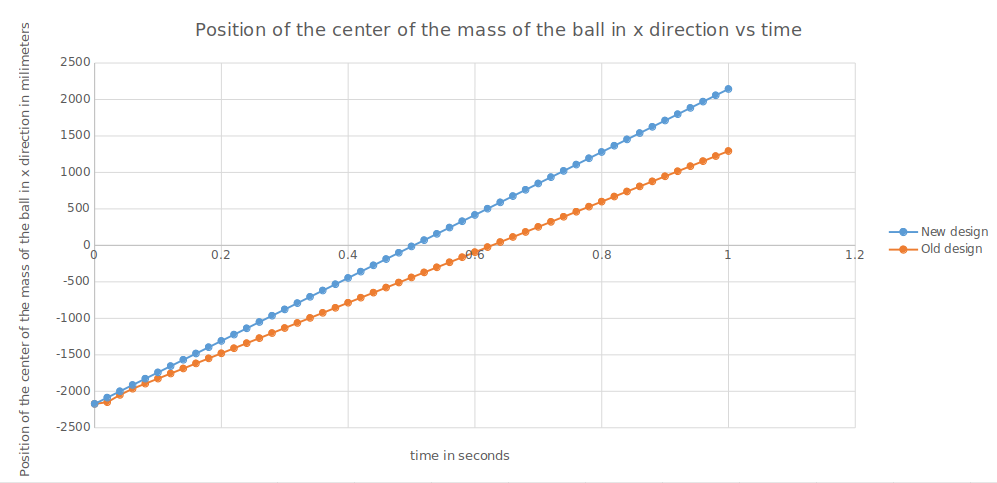
\includegraphics[width=0.8\textwidth]{images/CHIP_POS_PLOT.png}
	\caption{Position time graph for a ball being kicked by the new chip kicker (Blue)and old chip kick (Orange)}
	\label{fig:NEWOLDPLOTBALL}
\end{figure}
\\

In conclusion, the new chip kicker can kick the ball further than the old one. The most important point here is that the new chip kickers design made its process of manufacturing much easier and faster. %Also new design of kicking device is in a way that it can be easily disassembled from the robot which makes its repair process much faster. Faster robot repairing means having more robots operate when the match is taking place.



